% Ubah judul dan label berikut sesuai dengan yang diinginkan.
\section{ARCHITECTURE}
\label{sec:arsitektur}

\subsection{Arsitektur Sistem}
\begin{figure}[H] \centering
  % Nama dari file gambar yang diinputkan
  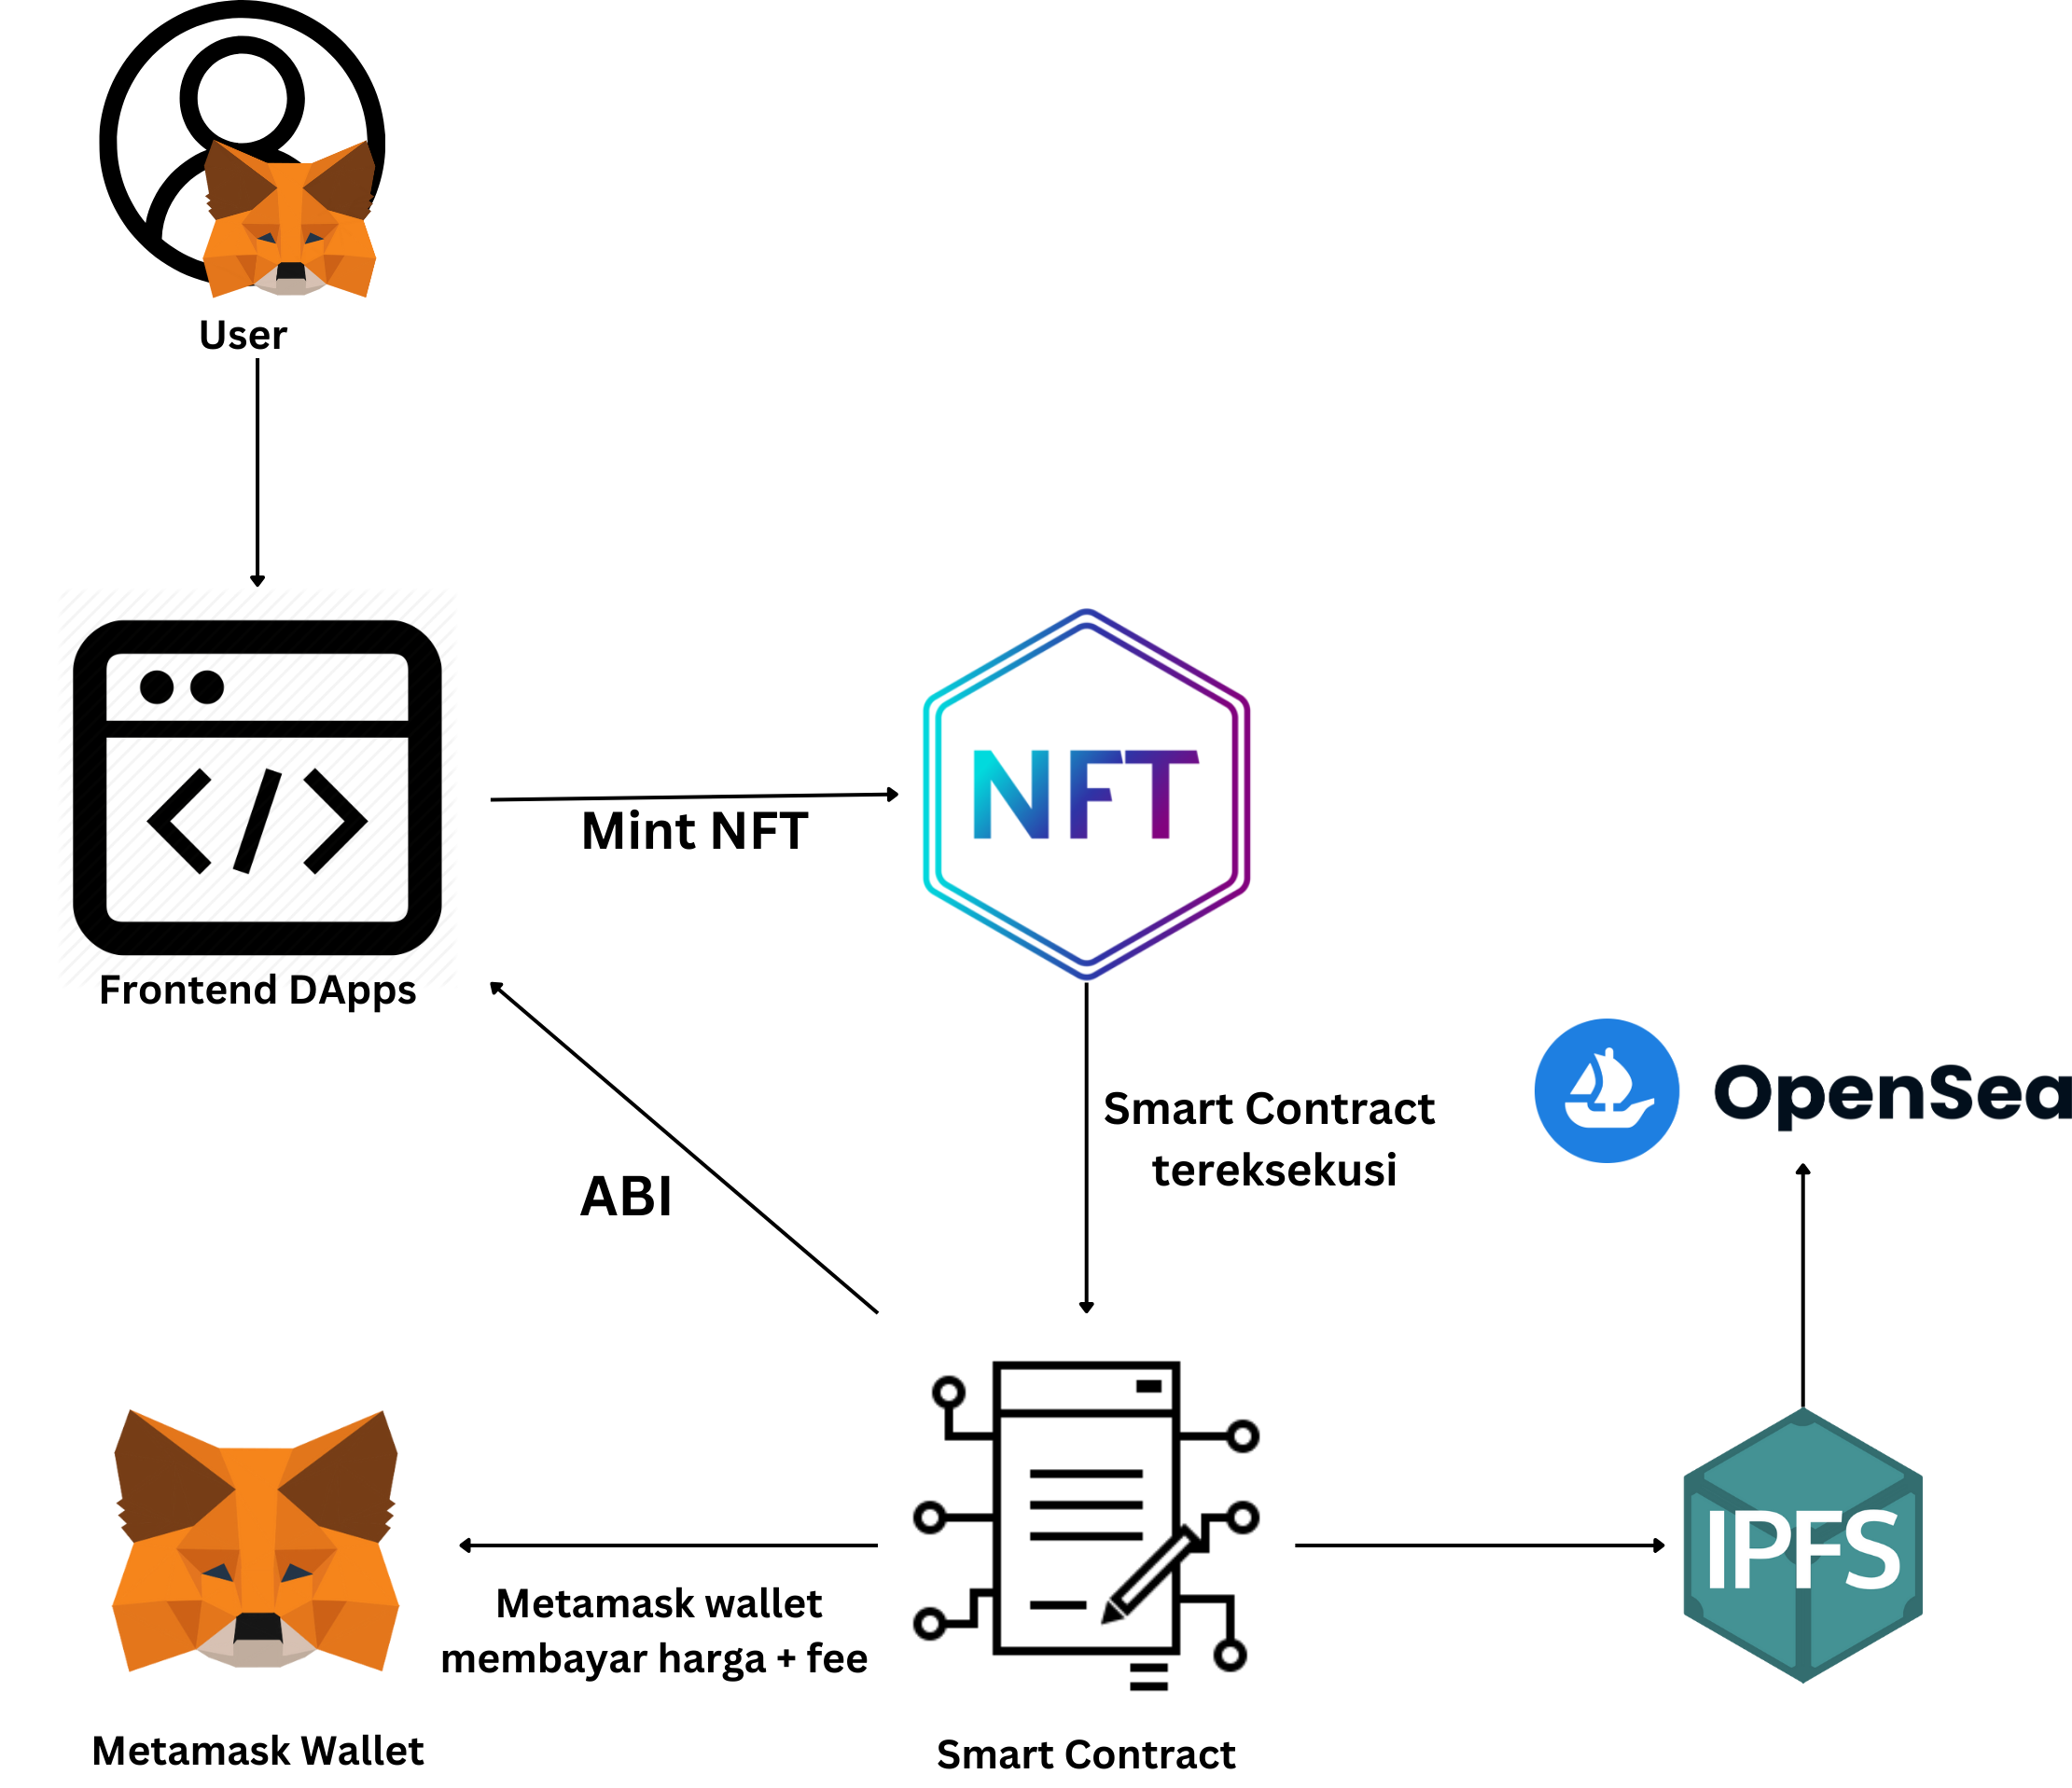
\includegraphics[scale=0.14]{gambar/desain_sistem_new.png}
  % Keterangan gambar yang diinputkan
  \caption{Desain sistem}
  % Label referensi dari gambar yang diinputkan
  \label{fig:desain_sistem}
\end{figure}

In the development of this smart contract system to function as intended by the author for completing this thesis, the author has designed a system architecture. In this system architecture, there is a role for the user who can become the owner of a token, and the user is the party with limited access to a token within a specified time. There is also a front end for the minting process of NFT tokens. To access the front end, both the owner and the user must connect using a Metamask wallet to interact.

On the front end, it connects with the smart contract when a user performs Minting, where the process involves the user uploading a digital asset they own to IPFS through a backend application, which then returns a Content Identifier (CID). A CID is a file address within IPFS used to access that file. The obtained CID is then uploaded to the blockchain network and becomes a token. Data about the available NFTs can be directly accessed by the front end through the smart contract on the blockchain.

% \vspace{0.5 cm}

\subsection{Proses Minting}
\begin{figure}[H] \centering
  % Nama dari file gambar yang diinputkan
  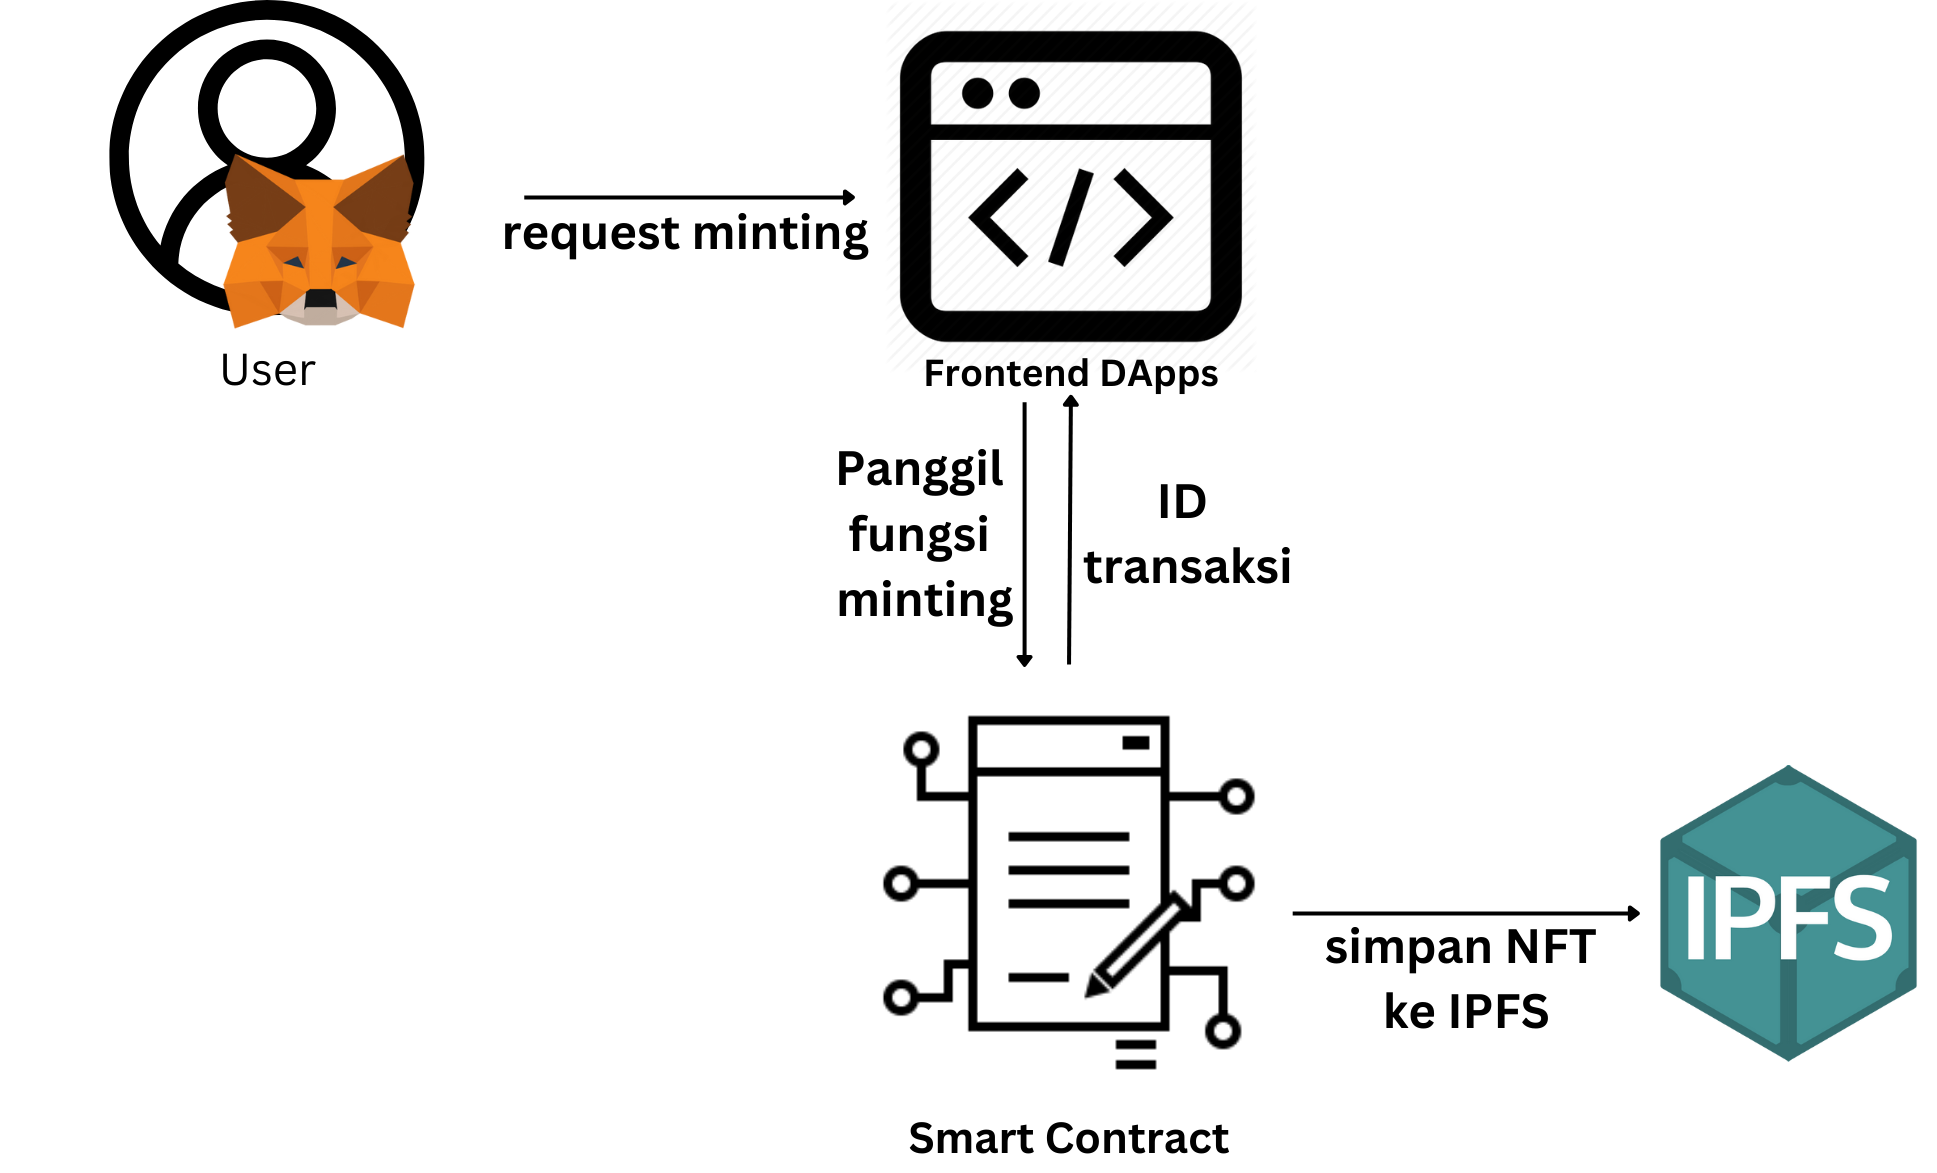
\includegraphics[scale=0.17]{gambar/proses_minting.png}
  % Keterangan gambar yang diinputkan
  \caption{Desain sistem}
  % Label referensi dari gambar yang diinputkan
  \label{fig:proses_minting}
\end{figure}

The minting process is the initial step where a new NFT is created on a platform. During this process, various important details about the NFT must be defined, including its name, description, category, available supply, and the visual asset representing the NFT, which could be a 2D image, 3D model, or video. The initial price, the collection that includes the NFT, and other attributes must also be determined. Once the minting process is complete, the data from the newly created NFT is stored in the InterPlanetary File System (IPFS), which allows for decentralized storage and access to data. This storage ensures that all related information, such as ownership recorded in the NFT’s attributes, can be accessed permanently and securely.

\subsection{Metode Yang Digunakan}
\begin{figure}[H] \centering
  % Nama dari file gambar yang diinputkan
  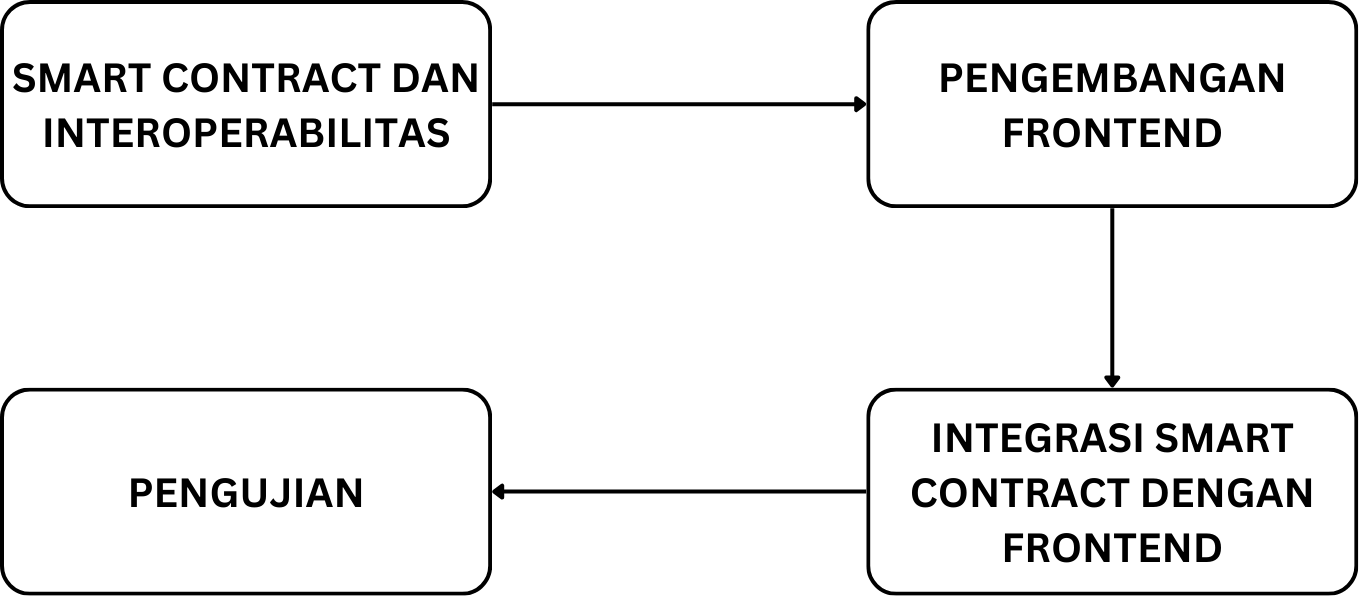
\includegraphics[scale=0.20]{gambar/metodologi_new.png}
  % Keterangan gambar yang diinputkan
  \caption{Metodologi Pengerjaan}
  % Label referensi dari gambar yang diinputkan
  \label{fig:metodologi}
\end{figure}

\subsubsection{Smart Contract dan Interoperabilitas}
In this stage, the author develops a smart contract system used for creating interoperable tokens using the Solidity programming language. This smart contract system acts as a bridge to process requests generated from user interactions on the frontend to the blockchain network. Upon compiling the smart contract, an Application Binary Interface (ABI) is generated, which can be used on the frontend for encoding and decoding data, allowing the frontend application to send precise instructions to the smart contract and understand the data returned by it. The smart contract developed by the author includes several core functions for the developed token.

\subsubsection{Pengembangan Frontend} 
To integrate a React application with the Ethereum blockchain, we utilize two primary libraries: ethers.js and web3.js. These libraries provide the necessary functionality to interact with the Ethereum blockchain, though they approach it slightly differently. Ethers.js is known for its minimalistic API and ease of use, which is particularly suitable for projects with simpler needs and a focus on reading and writing data to the blockchain. This library offers powerful functions for interacting with smart contracts, such as sending transactions, reading contract statuses, and handling event notifications.

\subsubsection{Integrasi Smart Contract dengan Frontend}
This stage enables applications built with React.js to interact directly with smart contracts deployed on the Ethereum network. To achieve this integration, we use the ethers.js library, which provides a clean and user-friendly interface for communicating with Ethereum.

Once the smart contract is developed and deployed, the ABI (Application Binary Interface) of the contract is used to construct a contract instance within the React application. The ABI allows the frontend to understand what functions are available in the smart contract, including the variables and data types used. With this information, ethers.js can invoke these functions, such as safeMint or transferOwnership, according to the logic defined in the contract.

\subsubsection{Pengujian}
This stage includes several steps for testing the smart contract, namely unit testing and integration testing.

\begin{itemize}
    \item Unit Testing
    This testing focuses on validating each component individually. In the context of a React.js frontend, this means testing components separately to ensure that they behave as expected. Unit testing is also conducted on the smart contract functions to verify their business logic, such as minting or token transfer functions. This testing is typically performed using the React framework for frontend and Hardhat for smart contracts.

    \item Integration Testing
    Following unit testing, the next step is integration testing, which ensures that all components in the application work well when combined. In the context of smart contract integration, this involves testing the interaction between the React.js frontend and the smart contract through ethers.js or web3.js. Integration testing helps detect issues in the data flow between the frontend and blockchain, including transaction validation and correct state updates.
    
\end{itemize}